\documentclass[aspectratio=169]{beamer}
\usepackage[english,russian]{babel}
\usepackage[utf8]{inputenc}
\usepackage{verbatim}
\usepackage{graphicx}
\usepackage{pgfpages}
\usepackage{ulem}
\usepackage{float}
\usepackage{amsmath}

\setbeameroption{hide notes}

\setbeamercolor{title}{fg=white}
\setbeamercolor{author}{fg=white}
\setbeamercolor{normal text}{fg=black}
\setbeamercolor{frametitle}{fg=black}
\setbeamercolor{item}{fg=red}
\setbeamercolor{block title}{fg=red}
\setbeamercolor{section in toc}{fg=red}
\setbeamercolor{footline}{fg=white}
\setbeamercolor{title in head/foot}{fg=white,bg=black}

\setbeamertemplate{navigation symbols}{}
\setbeamertemplate{headline}{
    
\includegraphics[height=1mm, width=\paperwidth]{wg-headline.png}
}

\setbeamertemplate{footline}{
    \begin{beamercolorbox}[ht=1.2em]{title in head/foot}
        {\footnotesize \hspace{1em}\inserttitle, \insertshortauthor}
    \end{beamercolorbox}
}

\begin{document}

\title{FOSDEM 2014}
\author{Maksim Melnikau}
\date{}

{
\title{
    \\
    {\huge FOSDEM 2014}
    \\
}

\usebackgroundtemplate{
\includegraphics[width=\paperwidth]{wg-end.jpg}}
\begin{frame}[plain]{}
    \titlepage
\end{frame}
}

\usebackgroundtemplate{
\includegraphics[width=\paperwidth]{wg-bg.jpg}}

{
\usebackgroundtemplate{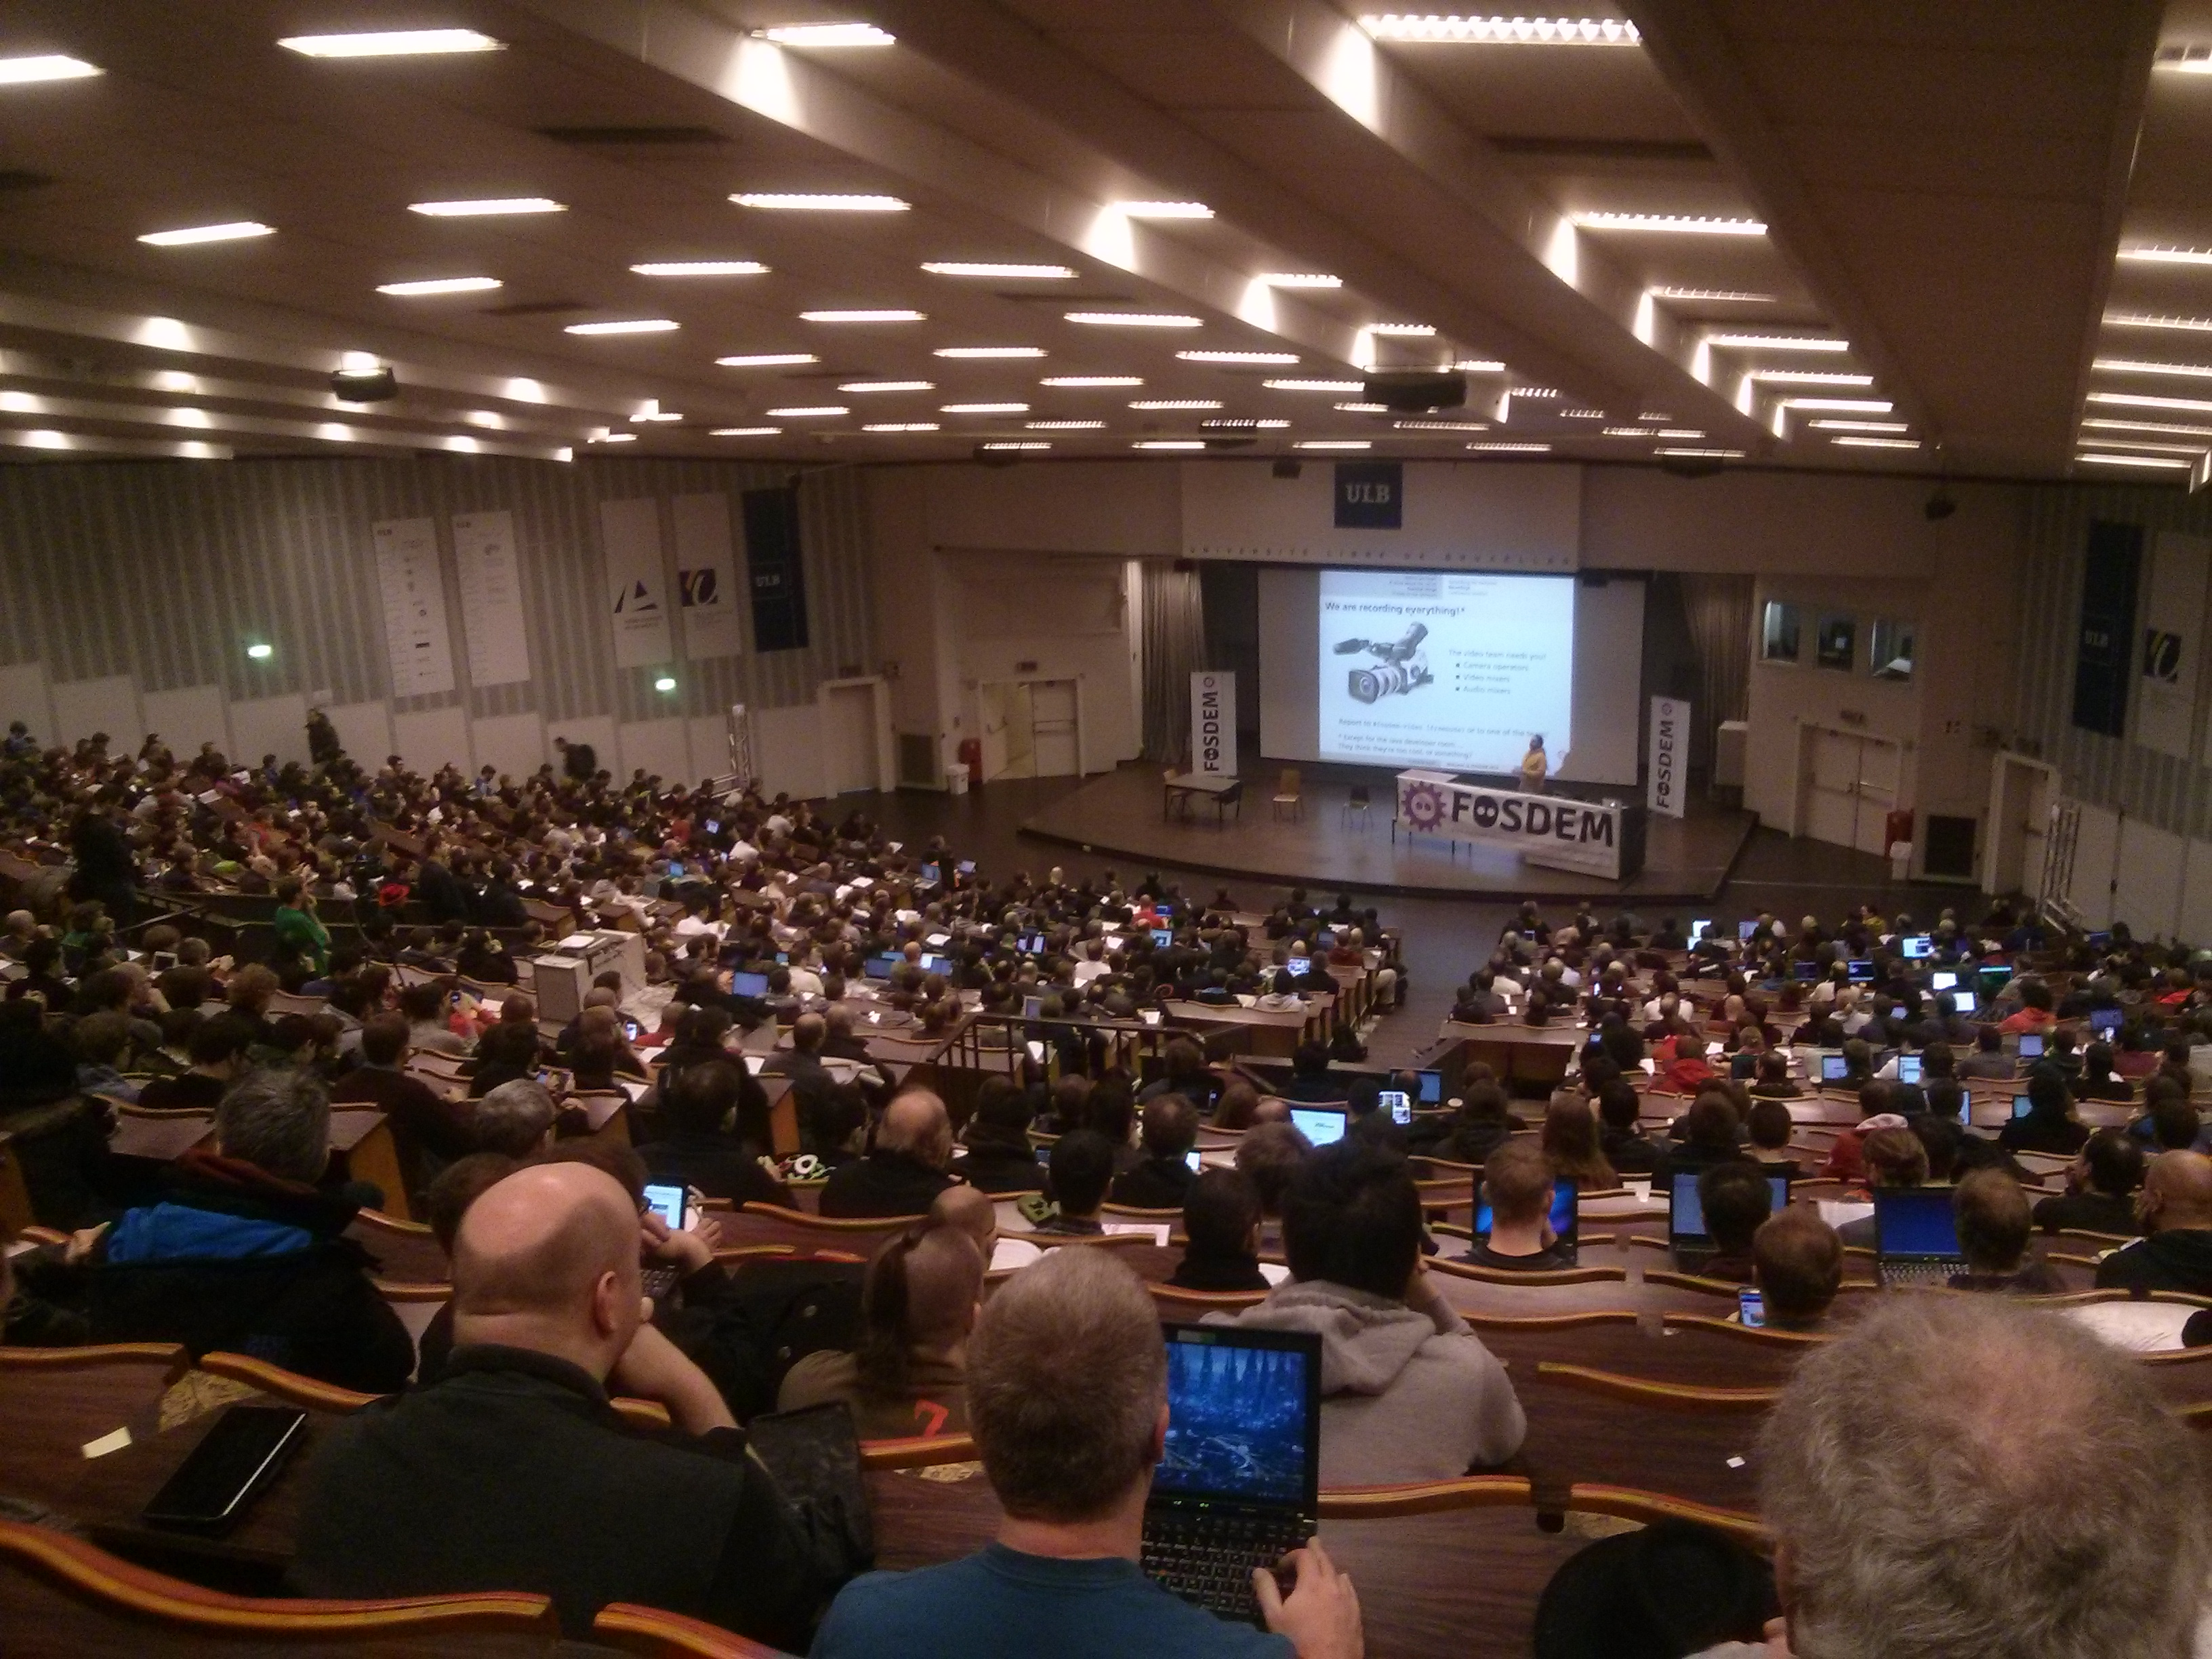
\includegraphics[width=\paperwidth]{fosdem.jpg}}
\begin{frame}[plain]{}
\end{frame}
}

\begin{frame}{How Find and Fix Million Grammar and Style Errors in Wikipedia}
  \begin{itemize}
  \item Wikipedia uses LanguageTool(LT) to find grammar errors
  \item LT - the next step after spell checking, LGPL, 10 regular commiters, Java+XML
  \item finds errors, but explanation sometimes wrong
  \item 68000 assembler (suggest: assemblers), if a is algebraic over K(suggest: an)
  \item LT: plain text => sentences => words => find part-of-speech and base form \\=> analyze sentences against error patterns
  \item LT patterns are easy to contribute in XML format, no java skills required
  \item LT supports many different languages including russian and belarusian
  \item grammar --- rules that describe how valid words, sentences, and texts looks like
  \item {\it Sorry for my bed English} grammatically is fine...
  \item \url{http://community.languagetool.org/feedMatches/list?lang=en}
  \item no need to stick to spell checking today - more powerful checks are available
  \end{itemize}
\end{frame}

\begin{frame}{kdbus, Lennart Poettering}
  \begin{itemize}
  \item D-Bus is powerful IPC: method call transactions, signals, properties,
        \\broadcasting, discovery, introspection, policy, activation, security,
        \\monitoring, expose APIs, File Description passing, language agnostic
  \item D-Bus has limitations: suitable only for control, not payload,
        \\inefficient; not available in early boot, initrd; baroque codebase
  \item if you try to solve problem with XML, you have two problems
  \item but still, D-Bus is fantastic, solves real problems
  \item kdbus suitable for large data (GiB!), zero-copy, optionally reusable,
        \\implicit timestamping; always available; no XML...
  \item 2 previous tries to get D-Bus in kernel grandiosely failed
  \end{itemize}
\end{frame}
 
\begin{frame}{miracast on Linux}
  \begin{itemize}
  \item miracast: HDMI over IP over Wifi
  \item ieee 802.11; wifi-p2p => wifi direct; wifi-display => miracast
  \item miracast: P2P transport setup, ip link auto discovery, A/V streams
  \item mirascast: many Linux wifi drivers not working (b43, brcmac, rtl818x, ath5k)
  \item some supposed to work (ath9k, brcmfmac, iwl-mvm)...
  \item known to work: iwl+mwm + intel wifi 7260 + wpa\_supplicant: git-78f79 ...
  \item HDMI over IP is RTSP + RTP + h264 + audio + mpeg2-TS
  \item Additional Features: PTP, HDCP, UIBC, split-sink
  \end{itemize}
\end{frame}

\begin{frame}{Sailfish and Jolla}
  \begin{itemize}
  \item half people at sailfish talk have Jolla device already
  \item Jolla: recovery mode, fastboot, unlocked bootloader, flash own kernels, full root
  \item sailfishos: systemd, gcc, btrfs, gstreamer, wayland, qt5
  \item Jolla not contribute to: L\&F UI, 3rd party closed source drivers, some NDA stuff
  \item \url{https://together.jolla.com/questions/} 
  \item contribute to sailfishos: contribute to nemo, mer, and a lot of upstream projects!
  \item libhybris - leverage existing Android hardware adaptation
  \item libhybris - port Android/bionic linker to glibc environment
  \item load glibc and bionic to address space of process --- works for almost all cases
  \item android\_dlopen("libEGL.so") - we could wrappers that accessed the android ones
  \item libhybris today used by Jolla/SailfishOS, Intel/Tizen, Canonical/Ubuntu
  \end{itemize}
\end{frame}  
  
\begin{frame}{Fedora.Next}
  \begin{itemize}
  \item Fedora.Next split to Workstation, Server, Cloud
  \item Fedora Workstation --- GUE for Students, Developers, etc ...
  \item Fedora Server --- headless {\it pet} server, server roles, IaaS Host,
        \\stable platform for critical infrastructure
  \item Fedora Cloud --- cloud image {\it cattle} server, scale-out, packaged images for clouds
  \item Fedora has so many infrastructure problems: bugs, reviews, build system, etc ...
  \end{itemize}
\end{frame}

\begin{frame}{FOSDEM network, NAT64 and DNS64}
  \begin{itemize}
  \item FOSDEM had ipv6-only wifi network by default
  \item but too many people escaped to fosdem-dualstack
  \item IPv4 has run out, IPv5 never made it to public use, so IPv6
  \item there was a war in begging of IPv6: 64bit vs unlimited!
  \item clients, content, carriers, applications, hardware - nobody want to do first step
  \item World IPv6 day - lets turn it on and see what breaks
  \item google, facebook, yahoo, youtube, netflix, akamai and many more run ipv6 today
  \item different countries enables ipv6 one by one - France, Germany, Belgium etc
  \item if you run NAT anyway - why not unable IPv6 and use NAT64 and DNS64 ?!
  \item we can hide a complete legacy internet in a /96!
  \item Nexus(Android) could not get ipv6 only address
  \item FOSDEM'14 --- first general-purpose conference which has ipv6 network by default
  \end{itemize}
\end{frame}

\begin{frame}{KDE Connect}
  \begin{itemize}
  \item fuse your devices as mush as possible and desirable
  \item protocol: json based, medium abstracted, easy extended, easy implemented
  \item notifications, actions, battery, MPRIS2, send files and urls
        \\clipboard synchronization, encryption, ...
  \item Qt => libconnect => server => plugins => D-Bus => plasma, kcm, apps
  \end{itemize}
\end{frame}  
  
\begin{frame}{GPU Offload on Wayland}
  \begin{itemize}
  \item render-nodes --- render without authentication to DRM master
  \item 1080p buffer with 60fps is 480MB/s, PCI express is 4GB/s, thunderbolt is 1GB/s
  \item tiling --- special pixel ordering optimized to exploit local spatial coherence
        \\--- good for performance
  \item GPU offload with X DRI2: DDX per device/provider, configure with xrandr
  \item two displays: A and B, two cards: 1 connected to A, 2 connected to B
        \\--- classic nvidia optimus layout
  \item wayland gpu offload: shutdown the dedicated GPU when unneeded works now
  \item XWayland: wlglamor, X linked to Wayland compositor - no need for gpu offloading
  \end{itemize}
\end{frame} 

\begin{frame}{Wine User Experience}
  \begin{itemize}
  \item once a year somebody writes at wine forum what "everything is work, you rock!"
  \item Ubuntu still ships 1.4.x wine version, why?!
  \item common problem when you answer to user question:
        \\if user hides, you don't know why: does everything work, user give up or died ...
  \end{itemize}
\end{frame} 
 
\begin{frame}{Performance of Wine and Graphical Drivers}
  \begin{itemize}
  \item command stream multi thread (CSMT) - move most d3d work into separate thread
  \item better CPU utilization => 2x performance (in theory)
  \item easy synchronization in multi-threaded games, even bigger performance gains
        \\3x in CoD 4:MW, btw Windows does the same thing
  \item wine CSMT improvements - some games faster on wine than on windows
  \item CSMT brings better performance mostly on fast systems like 460gtx + i7 ...
  \item drivers don't like to be called from two threads without looking
        \\even with separate contexts
  \item CSMT and NVIDIAS's threaded opt - essentially the same thing
  \item CSMT wine next steps: upstream, improve data streaming, reduce draw overhead in wine, wine performance outside d3d ...
  \item wine could have a big problems running on wayland natively
        \\--- many windows apps rely on window posistions for example
  \end{itemize}
\end{frame}  
  
\begin{frame}{Persistant Storage}
  \begin{itemize}
  \item file system performance: maximize throughput or latency?
        \\target embedded, power consumption or performance?
  \item high bandwidth has been the traditional focus --- backup, streaming video, etc
  \item SSD's made life more complicated --- not too painful at first, plaggued in
  \item PCI-e SSD devices turn up the heat
        \\opened a lot of other bottlenecks in Linux Storage Stack --- 1 million IOPS/device
  \item a single file system is easy for users and applications, and can perform better
  \item wow! fsck which works more than week!
  \item persistent memory - a variety of new technologies are coming from multiple vendors
        \\--- Linux need to be (mostly) technology neutral
  \item SNIA - Storage Network Industry Association, Working Group on NVM.
  \item SMR and PM together - interesting workload for out future
  \item normally block size limit is 4k, storage hardware often have very large - 64k
  \item PS --- you will never ever wait for storage anymore, CPU will be bottleneck
  \end{itemize}
\end{frame} 

\begin{frame}{Concurrent Programming Made Simple - Transaction Memory}
  \begin{itemize}
  \item shared memory (synchronization) + Transactions = Transaction memory (TM)
  \item TM --- programming abstraction, declare which code sequences are atomic
  \item TM is still rather new - standartization for C/C++ started 5 years go
        \\GCC has support since 4.7, HW implementations --- Haswell
  \item {\it \_\_transaction\_atomic \{ if (x<10) y++; \}} - code must be transaction-safe
  \item extend the C11/C++11 memory model --- all transactions totally ordered
  \item GCC: compiler --- ensure atomicity guarantee (at compile time)
  \item GCC: TM runtime library (libitm) => enforces atomicity o transactions at runtime
        \\(contains SW-only implementation)
  \item performance: it's a tool, not magic - {\bf useful balance}, implementations are wip
  \item single-thread performance: STM slower than sequential, HTM equals
        \\in multi-thread: both STM and HTM scales well
  \item TM, use it: {\it gcc -fgnu-tm}, report bugs and dive into libitm / GCC
  \item eventually consistency --- is not consistency at all
  \end{itemize}
\end{frame}

{
\setbeamertemplate{footline}{}
\setbeamercolor{frametitle}{fg=white}
\setbeamercolor{normal text}{fg=white}
\setbeamercolor{block title}{fg=white}
\setbeamercolor{block body}{fg=red}

\usebackgroundtemplate{
\includegraphics[height=\paperheight]{wg-end.jpg}}
\begin{frame}{Thank You. Questions}
    \begin{block}{Maksim Melnikau}
    \par \url{mailto:maxposedon@gmail.com}
    \par \url{https://plus.google.com/+MaksimMelnikau}
    \par \url{https://twitter.com/max\_posedon}
    \par \url{https://fosdem.org/2014/}
    \par \url{https://www.languagetool.org/}
    \par \url{http://lwn.net/Articles/580194/}
    \par \url{http://www.freedesktop.org/wiki/Software/openwfd/}
    \par \url{http://jolla.com/}
    \par \url{http://fedoraproject.org/wiki/Fedora.next}
    \par \url{http://en.wikipedia.org/wiki/NAT64}
    \par \url{https://fosdem.org/2014/schedule/event/kde\_connect/}
    \par \url{http://wayland.freedesktop.org/}
    \par \url{http://www.winehq.org/}
    \end{block}
\end{frame}
}

\end{document}
